\documentclass[UTF8,a4paper,zihao=-4]{ctexart}
%\usepackage{hyperref}%生成目录
\usepackage[bookmarks=true,colorlinks,linkcolor=black]{hyperref} %生成引用去掉框框
\usepackage[hmargin={3 cm,3 cm}]{geometry}%更改页面尺寸
\usepackage{graphicx}
\usepackage{amsmath}
\usepackage{amssymb}
\usepackage[]{enumitem} % 列表
\usepackage[numbers,sort&compress]{natbib} %参考文献以数字表示 且压缩如[1,2,3,4,5]->[1-5]
\usepackage{subfig}
\usepackage[justification=centering]{caption}

%\raggedbottom%顶部对齐,底部留空白
%\flushbottom% 分散对齐,default
\pagestyle{plain} %去掉页眉

\bibliographystyle{ieeetr}
\graphicspath{{pic/}{../pic/}} % {../pic/}为include,input


\begin{document}
\tableofcontents
\title{面向毫米波应用的无源元件建模}
\author{刘念宏{} 崔文普{} 付军}
\date{}%保持空白,去掉日期
\maketitle
%abstract
\noindent%段首不缩进
{\heiti 摘要:}此工作针对文献\cite{brinkhoff2008scalable}提出的毫米波无源元件建模提参方法进行改进,提出
了简单有效的电磁场仿真去嵌入方法。基于电磁场仿真(仿真参数通过测试数据校
准)得到的无源元件S参数,经去嵌入后,提取模型等效电路的参数,此等效电路模型
和SPICE兼容。依据上述建模提参方法,编写了一套适用于微带线CPW--GCPW的通
用建模提参程序。实现了0.5--100GH频段内CPW信号线长度、信号线宽度以及信号 
线和侧壁间距三个自由度同时可缩放模型,模型结果和45nm CMOS工艺流片结果对
比验证。
\indent

%1.	建模提参理论分析
\section{建模提参理论分析}
\subsection{新型电感传输线模型}
本方法主要参考文献\cite{brinkhoff2008scalable}中的工作并做一定改进。受趋肤效应、衬底漏电等效应的影响电感和传输
线等无源元件的特性阻抗和传播常数等参数是与频率相关的量。单位长度电感和传输线模型
可用图\ref{fig:RLGC}所示电路模型等效,图\ref{fig:RLGC}所示单位长度传输线等效电路模型
中的RLGC参数与频率无关,无法表示在毫米波应用下无源元件RLGC特性参数与频率相关
这一以特性,为了表示这一特性,需要对RLGC模型进行拓展。
\begin{figure}[t]
  \centering
  \includegraphics{RLGC.jpg}
  \caption{单位长度传输线等效电路模型}\label{fig:RLGC}
\end{figure}
\par
单$\pi$和$2\pi$模型是传输线和电感的常用模型,但是这两个模型的难以计算解析解、
需要通过算法调整优化、较难准确提取,模型结果难以和仿真或是测试结果拟合上,
且单$\pi$模型适用频率为10GHz以下\cite{yue1998chip},$2\pi$适用频率60GHz以下\cite{dickson200530},此两个模型的模型参数可放缩公式也难以建立。
\par
基于以上原因,文献\cite{brinkhoff2008scalable}提出了图\ref{fig:RLGC}所示的新型传输线和电感模型来拟合RLGC参数,此模型为经验模型,
所有模型参数均与频率无关。模型由串联部分和并联部分组成,串联部分与模型本身电感以及串联电阻损耗有关,
并联部分与模型对地电容以及对地电导有关。此经验模型的提出基于三方面的考虑:
%\begin{itemize}
%  \item 目前不存在一个物理模型能够描述直流到毫米波这么宽频段内的传输线和电感的频率特性;
%  \item 物理模型的参数的准确提取是一个困难的事;
%  \item 物理模型仅仅适用物理结构的器件,经验模型的通用性更广泛;
%\end{itemize}

\begin{enumerate}[itemsep=1pt, topsep=12pt, partopsep=0pt,label={(\arabic*)}] %设置间距
  \item 目前不存在一个物理模型能够描述直流到毫米波这么宽频段内的传输线和电感的频率特性;
  \item 物理模型的参数的准确提取是一个困难的事;
  \item 物理模型仅仅适用物理结构的器件,经验模型的通用性更广泛;
\end{enumerate}

\begin{figure}[htb]
  \centering
  \includegraphics[width=12cm]{paper_model.jpg}
  \caption{新型传输线和电感模型}\label{fig:paper_model.jpg}
\end{figure}
\par
图 \ref{fig:paper_model.jpg}中的模型在直流下没有对地的电导,就实际情况而言是不太合理的,
因此对图\ref{fig:paper_model.jpg}所示模型添加了对地电导,改进后的模型如图 \ref{fig:newmodel}所示。

\begin{figure}[htb]
  \centering
  \includegraphics[width=12cm]{newmodel.jpg}
  \caption{改进后的新型传输线和电感模型}\label{fig:newmodel}
\end{figure}

\subsection{模型参数提取}
为了获得可放缩的模型,需要大量的模型来确定放缩公式,基于时间和成本的考虑,
通过实际器件的测试数据校正电磁场仿真参数,通过电磁场仿真获得大量模型仿真结果。
使用电磁场仿真的结果对器件进行建模和参数提取,最后将其结果和测试数据进行对比验证。
\par
此模型是用来拟合单位器件长度RLGC参数,器件单位长度RLGC参数可通过电磁场得到S参数后转换而来\cite{eisenstadt1992s},
器件单位长度RLGC参数是与频率相关的。
\par
图 \ref{fig:newmodel}模型中,串联部分和并联部分模型参数提取可分开进行。


\subsubsection{串联部分的模型参数提取}
串联部分由直流电阻$R_0$、高频电感$L_0$和n个$R-L$并联网络组成。第k个$R-L$并联网络参数和第k个角频率$\omega_{sk}$满足如下关系:
\begin{equation}\label{equ:omegas}
  \omega_{sk}=\frac{R_k}{L_k}
\end{equation}

对于由n个$R-L$并联网络组成的模型,其串联部分整体电阻和电感计算可得:
%\begin{equation}\label{equ:R_omega}
%  R_{omega}=R_0+\sum_{k=1}^{n} \frac{R_k (\frac{\omega}{\omega_{sk}})^2} {{1+({\frac{\omega}{\omega_{sk}}})^2}}
%\end{equation}

\begin{align}
  R(\omega)&=R_0+\sum_{k=1}^{n} \frac{R_k (\frac{\omega}{\omega_{sk}})^2} {{1+({\frac{\omega}{\omega_{sk}}})^2}}  \label{equ:R_omega} \\
  L(\omega)&=L_0+\sum_{k=1}^{n} \frac{L_k} {{1+({\frac{\omega}{\omega_{sk}}})^2}}  \label{equ:L_omega}
\end{align}

对于0--100GHz频段内取$n=3$便能实现较好的拟合,选择合适角频率使其满足:
\begin{equation}
 ( \frac{\omega_{s2}}{\omega_{s1}})^2, \ {( \frac{\omega_{s2}}{\omega_{s1}})^2}\gg 1
\end{equation}

假设$R_1,R_2,R_3$具有相同的数量级,$L_1,L_2,L_3$具有相同数量级,则式\ref{equ:R_omega}和\mbox{式 \ref{equ:L_omega}}可化简为:
\begin{gather}
  R(\omega_{s1})=R_0+\frac{R_1}{2}  \label{equ:ss1} \\
  R(\omega_{s2})=R_0+R_1+\frac{R_2}{2} \label{equ:ss2}  \\
  R(\omega_{s3})=R_0+R_1+R_2+\frac{R_3}{2} \label{equ:ss3} \\
  L(\omega_{s1})=L_0+\frac{R_1}{2\omega_1}+\frac{R_2}{\omega_2}+\frac{R_3}{\omega_3} \label{equ:ss4} \\
   L(\omega_{s2})=L_0+\frac{R_2}{2\omega_2}+\frac{R_3}{\omega_3} \label{equ:ss5}
\end{gather}

通过求解式 \ref{equ:omegas},式 \ref{equ:ss1}--式 \ref{equ:ss5}组成的方程组,
可求得模型串联部分参数$R_0  ,R_1,R_2$, $R_3$, $L_0$, $L_1$, $L_2$, $L_3$  。

\subsubsection{并联部分的模型参数提取}
并联部分由直流对地电导$G_0$、高频对地电容$C_0$和n个$C-G$串联网络组成。
第k个$C-G$串联网络参数和第k个角频率$ω_{pk}$满足如下关系:
\begin{equation}
  \omega_{pk}=\frac{G_k}{C_k} \label{equ:omegap}
\end{equation}

对于由n个$C-G$串联网络组成的模型,其并联联部分整体电阻和电感计算可得:
\begin{align}
  G(\omega)&=G_0+\sum_{k=1}^{n} \frac{G_k (\frac{\omega}{\omega_{pk}})^2} {{1+({\frac{\omega}{\omega_{pk}}})^2}}  \label{equ:G_omega} \\
  C(\omega)&=C_0+\sum_{k=1}^{n} \frac{C_k} {{1+({\frac{\omega}{\omega_{pk}}})^2}}  \label{equ:C_omega}
\end{align}

对于0-100GHz频段内取n=3便能实现较好的拟合,选择合适角频率使其满足:
\begin{equation}
 ( \frac{\omega_{p2}}{\omega_{p1}})^2, \ {( \frac{\omega_{p3}}{\omega_{p2}})^2}\gg 1
\end{equation}

假设$G_1,G_2,G_3$具有相同的数量级$C_1,C_2,C_3$具有相同数量级,则\mbox{式\ref{equ:G_omega},式\ref{equ:C_omega}}可化简为:
\begin{gather}
  G(\omega_{s1})=G_0+\frac{G_1}{2}  \label{equ:pp1} \\
  G(\omega_{s2})=G_0+G_1+\frac{G_2}{2} \label{equ:pp2}  \\
  G(\omega_{s3})=G_0+G_1+G_2+\frac{G_3}{2} \label{equ:pp3} \\
  C(\omega_{s1})=C_0+\frac{G_1}{2\omega_1}+\frac{G_2}{\omega_2}+\frac{G_3}{\omega_3} \label{equ:pp4} \\
   C(\omega_{s2})=C_0+\frac{G_2}{2\omega_2}+\frac{G_3}{\omega_3} \label{equ:pp5}
\end{gather}

通过求解式 \ref{equ:omegap},式 \ref{equ:pp1}--式 \ref{equ:pp5}组成的方程组,
可求得模型串联部分参数$G_0  ,G_1,G_2$, $G_3$, $C_0$, $C_1$, $C_2$, $C_3$  。

\subsubsection{模型参数优化}
文献\cite{brinkhoff2008scalable}中,直接取$\omega_{p1}$,$\omega_{s1}=2π×1GHz$,$\omega_{p2}$,$\omega_{s2}=2π×10GHz$,$\omega_{p3},\omega_{s3}=2π×100GHz$
即可实现较高的模型拟合精度,但实际发现对$\omega_{si}$,$\omega_{pi}$如此取值的话只针对特殊结构特殊工艺下的
模型有效,对于一般的模型会带来非常大的拟合误差。为了实现拟合误差的最小化需要对$\omega_{si}$,$\omega_{pi}$进行调整优化。
为了简化问题,取$\omega_{p1}$,$\omega_{s1}=2π×1GHz$,$\omega_{p3},\omega_{s3}=2π×100GHz$固定不变,$\omega_{p2}$,$\omega_{s2}$作为优化变量。
由于模型串联部分和并联部分的数学形式完全一样,其优化算法也是一样的,$\omega_{s2}$,$\omega_{p2}$的优化过程完全一致,下面以优化$\omega_{s2}$为例进行说明。
优化的目标是使模型拟合误差最小化,采用相对误差作为误差衡量标准,单位长度R、L拟合误差函数如公式\ref{equ:err_RL}:

\begin{align}\label{equ:err_RL}
Err({\omega _{s2}}) =\sum\limits_{i = 1}^m {{W_{Ri}}} \left| {1 - \frac{{{R_0} + \frac{{{R_1}{{\left( {\frac{{{\omega _i}}}{{{\omega _{s1}}}}} \right)}^2}}}{{1 + {{\left( {\frac{{{\omega _i}}}{{{\omega _{s1}}}}} \right)}^2}}} + \frac{{{R_2}{{\left( {\frac{{{\omega _i}}}{{{\omega _{s2}}}}} \right)}^2}}}{{1 + {{\left( {\frac{{{\omega _i}}}{{{\omega _{s2}}}}} \right)}^2}}} + \frac{{{R_3}{{\left( {\frac{{{\omega _i}}}{{{\omega _{s3}}}}} \right)}^2}}}{{1 + {{\left( {\frac{{{\omega _i}}}{{{\omega _{s3}}}}} \right)}^2}}}}}{{R\left( {{\omega _i}} \right)}}} \right|  & \notag \\
+\sum\limits_{i = 1}^m {{W_{Li}}} \left| {1 - \frac{{{L_0} + \frac{{{L_1}{{\left( {\frac{{{\omega _i}}}{{{\omega _{s1}}}}} \right)}^2}}}{{1 + {{\left( {\frac{{{\omega _i}}}{{{\omega _{s1}}}}} \right)}^2}}} + \frac{{{L_2}{{\left( {\frac{{{\omega _i}}}{{{\omega _{s2}}}}} \right)}^2}}}{{1 + {{\left( {\frac{{{\omega _i}}}{{{\omega _{s2}}}}} \right)}^2}}} + \frac{{{L_3}{{\left( {\frac{{{\omega _i}}}{{{\omega _{s3}}}}} \right)}^2}}}{{1 + {{\left( {\frac{{{\omega _i}}}{{{\omega _{s3}}}}} \right)}^2}}}}}{{L\left( {{\omega _i}} \right)}}} \right| &
\end{align}
\begin{equation}\label{equ:weight}
  \sum_{i=1}^{m}W_{Ri}+\sum_{i=1}^{m}W_{Li}=1 \qquad    W_{Ri}\geq0,W_{Li}\geq0
\end{equation}

公式\ref{equ:err_RL}中m为电磁场仿真的频点数,$R(\omega_i)$和$L(\omega_i)$为各频点下图 \ref{fig:RLGC}单位长度电阻和电感值,$W_{Ri}$和$W_{Li}$为各频点的优化权重。
\par
误差函数的取值是离散的且需要考虑的取值点较少,可通过遍历的方法求得误差函数的最小值,找到最佳的$\omega_s2$以及模型参数$R_0$,$R_1$,$R_2$,$R_3$,$L_0$,$L_1$,$L_2$,$L_3$。
建模提参整个流程如图\ref{fig:process_flow}所示。
\begin{figure}[htb]
  \centering
  \includegraphics[scale=0.6]{process_flow.pdf}
  \caption{建模提参流程图}\label{fig:process_flow}
\end{figure}

\section{去除电磁场仿真端口效应}
理想无限长传输线各处均匀,实际电磁场仿真中由于硬件以及时间限制,实际电磁场仿真的模型长度有限。
由于电磁场仿真中端口和模型信号线本身的不连续性导致信号线上电场磁场分布不均匀。图 \ref{fig:e_field}中为
一200um长CPW的电场分布图,从图中可以看出模型电场中间部分分布均匀,而两端口处分布不均匀。
理想情况下,不同长度的CPW计算得到其单位长度RLGC值应该是相同的,由于端口效应的影响不同
长度的CPW计算得到其单位长度RL值如图\ref{fig:unit_RL2}所示,从图中可以看出其不同长度的CPW计算得到其
单位长度RL值与CPW模型长度相关。
\begin{figure}[htb]
  \centering
  \includegraphics[width=12 cm]{E_field.png}
  \caption{200um长CPW的电场分布图} \label{fig:e_field}
\end{figure}

\begin{figure}[htb]
\centering
  % Requires \usepackage{graphicx}
  \subfloat[单位长度R]{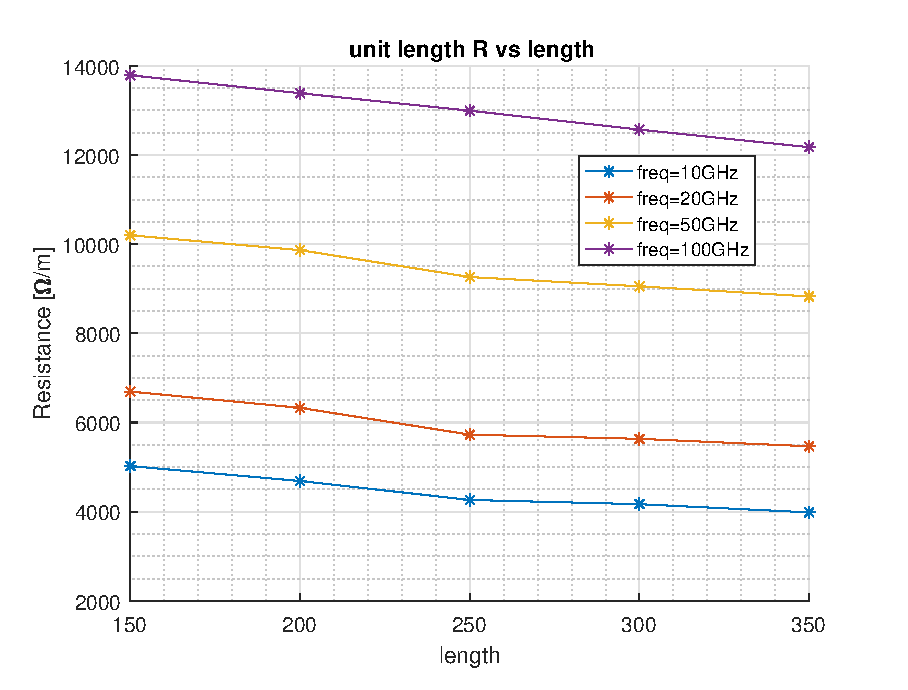
\includegraphics[width=7cm]{R_unit_len.eps}\label{fig:unit_R}}
 \hspace{0.1cm}
 %\qquad
  \subfloat[单位长度L]{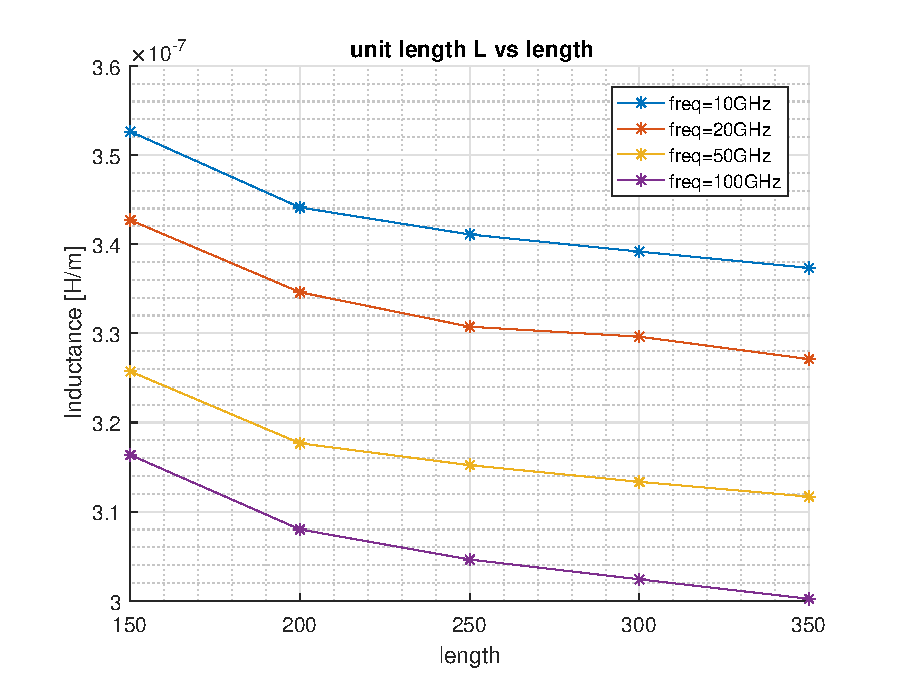
\includegraphics[width=7cm]{L_unit_len.eps}\label{fig:unit_L}}
  \vspace{0.5cm}
  \centering
   \caption{不同长度的CPW计算得到其单位长度RL值 \protect \\(CPW S=4um W=4um L=150um,200um,250um,300um,350um)} \label{fig:unit_RL2}
\end{figure}

为了得到模型本身的特性参数,需要去除端口效应的影响,基于此提出包含端口影响的等效电路模型,
如图\ref{fig:port},端口效应用串联R-L电路等效。R,L,G,C为无端口效应模型的本征参数,
$R_f$,$L_f$为端口效应电阻电感。按照图\ref{fig:port}端口效应对模型单位长度G、C没有影响,只对模型单位长度R、L的提取有影响。
\begin{figure}
  \centering
  \includegraphics[width=12cm]{port_influence.pdf}
  \caption{含端口效应的等效电路模型}\label{fig:port}
\end{figure}

以$R_t,L_t,G_t,C_t$,为模型总电阻、电感、电导、电容,有如下关系:
\begin{align}
  R_t &=R*len+2R_f  \label{equ:port_r}\\
  L_t &=L*len+2L_f \label{equ:port_l} \\
  G_t &=G*len  \label{equ:port_G}\\
  C_t &=C*len \label{equ:port_c}
\end{align}
   式\ref{equ:port_r}-- 式\ref{equ:port_c} 可转换为如下关系:
\begin{align}
  \frac{R_t}{len}&= R+\frac{2R_f}{len} \label{equ:port_r_new}\\
   \frac{L_t}{len}&= L+\frac{2L_f}{len} \label{equ:port_l_new} \\
   \frac{G_t}{len}&= G \label{equ:port_g_new} \\
  \frac{C_t}{len}&= C \label{equ:port_c_new}
\end{align}

从式\ref{equ:port_r_new}--式 \ref{equ:port_l_new}基于此端口效应模型可得到图\label{fig:unit_RL}所示结果,由于端口效应影响,
单位长度电阻、电感随着模型长度增加而减小。
\par
基于此端口效应模型以$1/len$为自变量,$R_t/len$为因变量做图,如图 2.4所示。
\begin{figure}[htb]\label{fig:1unit_RL}
\centering
  % Requires \usepackage{graphicx}
  \subfloat[单位长度R]{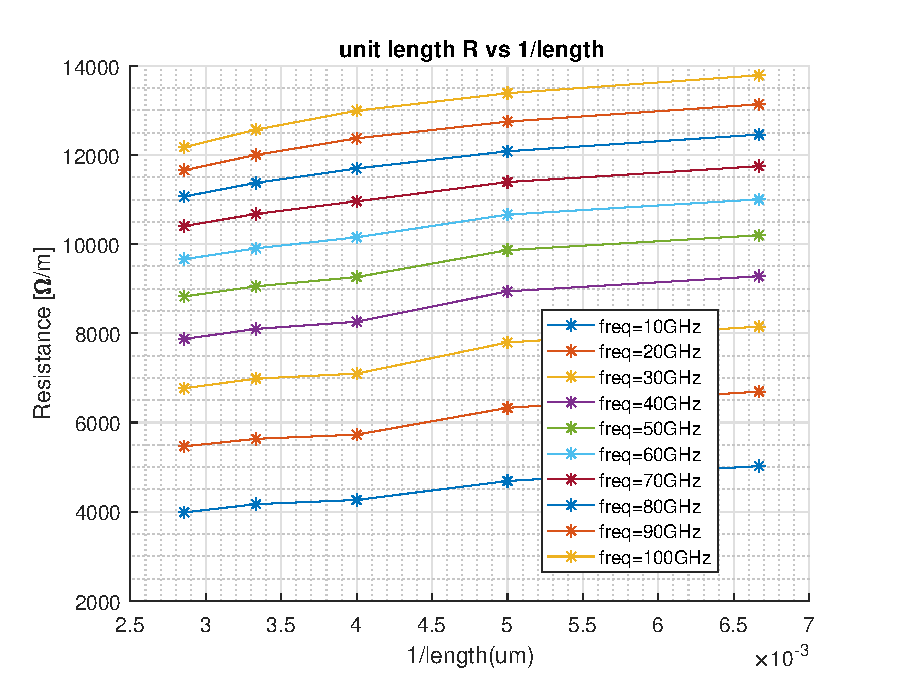
\includegraphics[width=7cm]{R_1unit_len.eps}\label{fig:1unit_R}}
 \hspace{0.1cm}
 %\qquad
  \subfloat[单位长度L]{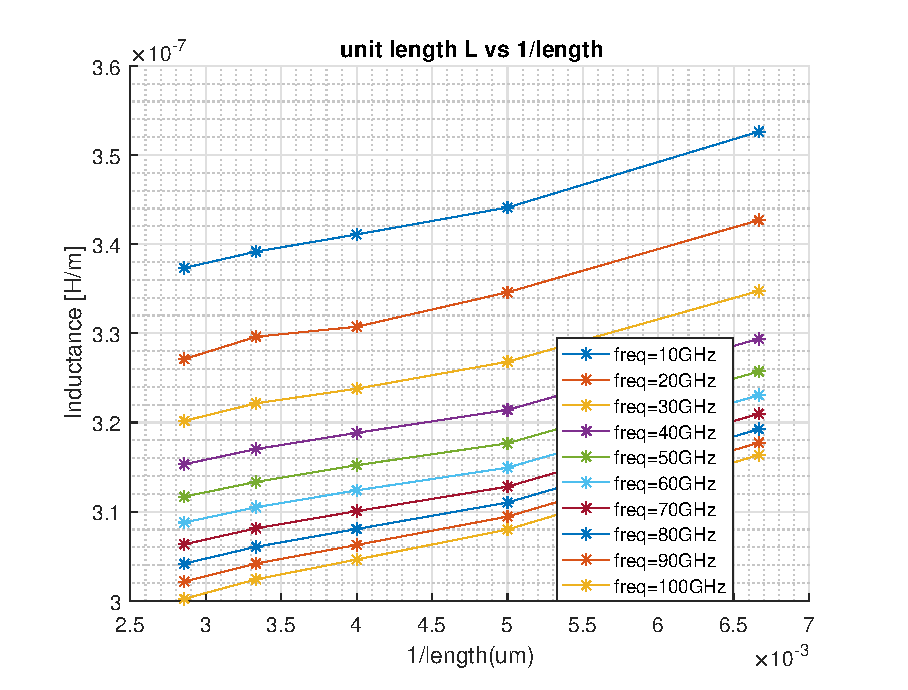
\includegraphics[width=7cm]{L_1unit_len.eps}\label{fig:1unit_L}}
  \vspace{0.5cm}
  \centering
   \caption{CPW模型单位长度电阻电感与模型长度的倒数的关系\protect \\(CPW S=4um W=4um L=150um,200um,250um,300um,350um)}
\end{figure}

结合式\ref{equ:port_r_new}--式 \ref{equ:port_l_new},通过最小二乘法做拟合直线,可提取模型本征单位长度\mbox{R、L}。


\section{	CPW建模提参以及可放缩模型}




\bibliography{myRef}



\end{document}
